\chapter{Three peak appearance in the Double Quantum Dot model.\label{chap:DoublePeak.}}

The DQD model is characterized by the formation of 
a new state that entangles the two Quantum dots through the leads. This produces an anti-ferromagnetic interaction between the QDs, commonly known
as Ruderman-Kittel-Kasuya-Yosida (RKKY) interaction \citep{ruderman_indirect_1954,yosida_magnetic_1957}. As consequense, two satelite peaks will emerge in the Density of States.  




To explain this phenomenon we will take a symmetric version of Hamiltonian \eqref{General model} with $2e_i =U_i =U $ , $t_i = t$ and $t_{dots} = 0$ for $i \in \{ 1,2 \}$. 
\begin{equation}
H =\sum_{i,k,\sigma}  \frac{U_i}{2}(d_{i \sigma}^{\dagger}d_{i \sigma}-1)^{2} + t(d_{+,\dw}+d^\dagger_{+,\dw})\gamma_1 + \Gamma_i(d^\dagger_{i\sigma}c_{k\sigma}+c^\dagger_{k\sigma}d_{i\sigma}).
\label{SymModel}
\end{equation}

The symmetry of the previous Hamiltonian is suitable to apply a base change of the form 
 
\[
  d_{+ , \sigma} = \frac{1}{\sqrt{2}} (d_{1\sigma} +d_{2\sigma}) \ , \ 
  d_{- , \sigma} = \frac{1}{\sqrt{2}} (d_{1\sigma} -d_{2\sigma}).
\]


These new operators satisfy the fermionic anti-commutation relations 
 \[ \{d_{\pm , \sigma}, d^\dagger_{\pm , \sigma}\} = 1 , \{ d_{\pm , \sigma}, d^\dagger_{\mp , \sigma}\} = 0,
\]
 so that the may be considered as fermion operators. All lineal terms in \eqref{SymModel} are trivially adapted to the new base. The repulsion potential 
$$\sum_{i} (\sum_{\sigma} d_{i \sigma}^{\dagger}d_{i \sigma}-1)^{2} = (\sum_{\sigma} d_{1 \sigma}^{\dagger}d_{1 \sigma}-1)^{2} + (\sum_{\sigma} d_{2 \sigma}^{\dagger}d_{2 \sigma}-1)^{2} . $$ 
gives rise to a non-trivial interaction between the new states. To find this interaction we define the particle number operator  
\[\hat{n}_{i,\sigma}:= d^\dagger_{i,\sigma}d_{i,\sigma}.\] 

So that 
\[\hat{n}_{1,\sigma}= \frac{1}{2} \left( \hat{n}_{+,\sigma} + \hat{n}_{-,\sigma} + d^\dagger_{+,\sigma}d_{-,\sigma} + d^\dagger_{-,\sigma}d_{+,\sigma} \right) = \frac{1}{2} \left( \hat{N}_\sigma + \hat{E}_\sigma \right),  \]
with $\hat{N} = \hat{n}_{+,\sigma} + \hat{n}_{-,\sigma}$ and $\hat{E}_\sigma = d^\dagger_{+,\sigma}d_{-,\sigma} + d^\dagger_{-,\sigma}d_{+,\sigma}. $ Similarly 

\[\hat{n}_{2,\sigma}= \frac{1}{2} \left( \hat{N}_\sigma - \hat{E}_\sigma \right).  \]
Hence 

\[\sum_{i} (\sum_{\sigma} d_{i \sigma}^{\dagger}d_{i \sigma}-1)^{2} = \left(\frac{\hat{N} +\hat{E}}{2}-1 \right) ^{2} + \left( \frac{\hat{N} -\hat{E}}{2}-1 \right)^{2} = \frac{\left( \hat{N}-2 \right)^2- \hat{E}^2}{2}, \]

with $\hat{N}=\sum_\sigma \hat{N}_\sigma $ , $\hat{E}=\sum_\sigma \hat{E}_\sigma $. Note that opeator $\hat{N}$ represents the total occupation number inside both dots. If this occupation is different than $2$ there is an imbalance between particles and dots that is punished by this term. The term $E^2$ is much more interesting since this one is the responsible for the emergence of satellite peaks in the DOS. To understand what it makes it is simple to observe its results when applied to a based ordered by $\vert + , - \rangle$. 
\[ \hat{E}^2 \vert \up , 0 \rangle =  \hat{E} \vert 0 , \up \rangle = \vert \up , 0 \rangle   \] 
\[ \hat{E}^2 \vert \up , \dw \rangle =  \hat{E} \left( \vert 0 , \up\!\dw \rangle + \vert \up\!\dw , 0 \rangle \right) = 2\vert \up , \dw \rangle - 2\vert \dw , \up \rangle  \]





The new Hamiltonian 
\begin{equation}
H = \sum_{\sigma}  \frac{U}{4}\left( \left( \hat{N}-2 \right)^2- \hat{E}^2 \right) + \frac{t}{\sqrt{2}} (d_{+,\dw}+d^\dagger_{+,\dw})\gamma_1 
 +  \frac{\Gamma}{\sqrt{2}}\sum_{ k}(d^\dagger_{+,\sigma}c_{k\sigma}+c^\dagger_{k\sigma}d_{+,\sigma})
\label{t+}
\end{equation}
is represented in \ref{fig:ExchangeMod}

% \begin{figure*}[h]
% \centering
% 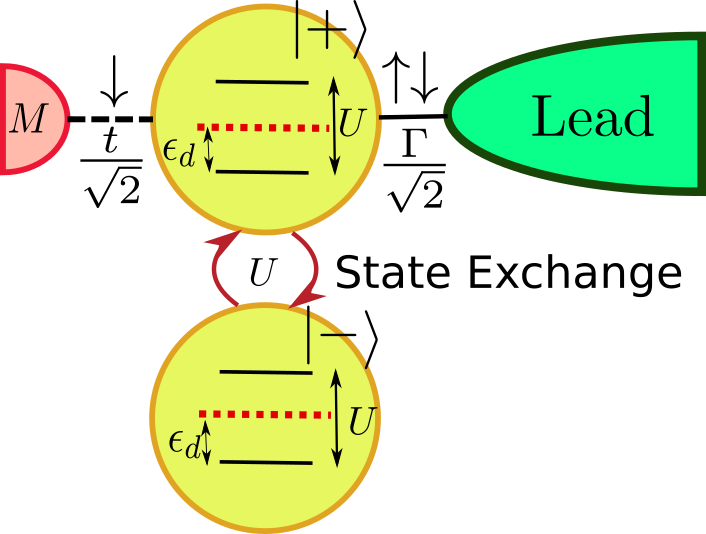
\includegraphics[scale=0.4]{IMAGES/ExchangeMod.png}
% \caption{\label{fig:ExchangeMod} General model.} 
% \end{figure*}




%\begin{equation}
%H = \sum_{i,k} \left(\epsilon_{d}+\frac{U}{2}\right)d_{\sigma}^{\dagger}d_{\sigma}+\frac{U_i}{2}(d_{\sigma}^{\dagger}d_{\sigma}-1)^{2} + t_i d_i+d^\dagger_i \gamma_1 + \Gamma_i(d_{\sigma}c_{\sigma})
%\end{equation}


We can explain this three-peak as the result of a new strong coupling interaction characterized by the spin exchange between both dots. 
%HERE COMES THE CHANGE OF BASIS 

In addition, the spin-up DOS at the Fermi energy grows faster than the spin-down DOS, breaking the initial spin-symmetry when $t_1=t_2=0$. At $t_1=t_2=0.02D$ the spin-up DOS at the fermi energy doubles the spin-down DOS which implies that the Majorana signature  is present in both dots. %I need to write what is this Majorana signature about. 
Indeed \ref{fig:MSig/Shift_t1=t2} shows that the relation $\frac{\rho_\up(0)}{\rho_\up(0)}$ increases continuously from $1$ to $2$. Note that the Majorana is completely attached when the coupling $t_1$ reaches the order of $0.01D$ .